% ****************************************************************************************************
% Chapter 9: Fairness, Age, and Compensated Shock
% ****************************************************************************************************

\chapter{Fairness, Age, and Compensated Shock}
\label{ch:fairness}

The operating curve from the previous chapter gives a hospital a menu of achievable trade-offs between overall accuracy and overall under-triage rate. A sensible question follows immediately: does every patient experience the same trade-off? When I report that my default operating point produces a $15.22\%$ under-triage rate, that average hides enormous variation across patient subgroups. Some populations are under-triaged at more than twice the overall rate; others at half. If the model is to be deployed, I need to know who the errors fall on.

This chapter is an audit of that question. I report the under-triage rates of my model across intersecting combinations of age, sex, and race, and I find a pattern that was not what I expected to find. The dominant axis of disparity is not race, and it is not sex. It is age, and specifically young age: the patients my model most often under-triages are in the 18--30 range. The finding is not an artefact of my particular modelling choices, it reflects a well-documented clinical phenomenon called compensated shock, in which young patients maintain apparently normal vital signs even when severely ill. The chapter closes with an attempt to correct the disparity through feature engineering, and with a surprising negative result from the previous chapter made explicit here: the safety threshold intervention that reduces overall under-triage does so at the cost of \emph{widening} the disparity between best-off and worst-off subgroups.

\section{The Structure of the Audit}

Fairness audits in clinical machine learning typically examine single demographic axes in isolation: under-triage rate by race, by sex, by age band. This is useful, but it conceals a structural problem. A model can appear fair on each individual axis while having large disparities at their intersections. A classic illustration is a hiring algorithm that is fair to men, fair to women, fair to Black candidates, and fair to white candidates, but systematically disadvantages Black women, the \emph{intersectional} subgroup. Single-axis fairness metrics cannot detect this pattern.

I ran an intersectional audit spanning three axes: age group (five bands: 18--30, 31--50, 51--65, 66--80, 80+), sex (M, F), and race (five aggregated categories: WHITE, BLACK, ASIAN, HISPANIC, OTHER). The audit computed the under-triage rate for every combination with at least 50 patients, yielding 57 subgroups in total. The full set is too large to display; I focus here on the pattern that emerged.

\begin{notebox}[A Caveat on Race Categories]
The five race categories I report are aggregated from a much richer set of self-reported values in MIMIC-IV-ED. The mapping from raw values (33 distinct strings including ``WHITE - RUSSIAN'', ``HISPANIC/LATINO - PUERTO RICAN'', ``ASIAN - CHINESE'', and many others) to my five categories was done through a simple dictionary lookup that matched only the canonical base strings. This means that subcategories were routed to ``OTHER'' rather than to their parent category: for example, the $13{,}913$ patients coded as ``HISPANIC/LATINO - PUERTO RICAN'' fell into ``OTHER'' rather than ``HISPANIC''. As a result, my ``HISPANIC'' category contains only $3{,}070$ patients rather than the much larger number a complete mapping would have produced, and similarly for the ``ASIAN'' and ``BLACK'' categories.

This flaw substantially undercounts minority populations and inflates the ``OTHER'' category. The findings I report below about age as the dominant disparity axis are robust to this issue, age effects are far larger than race effects in absolute terms, but the specific race-level numbers should be read with caution. A proper follow-up analysis would use a complete mapping.
\end{notebox}

\section{Patterns in the Audit}

The clearest pattern in the audit is that age, not sex or race, dominates the variation in under-triage rate. Before turning to the single-axis numbers, I note one observation from the full intersectional sweep: \emph{every} combination of age with other demographic variables that produced an under-triage rate meaningfully above the overall average fell in one of the two youngest age bands (18--30 or 31--50). No intersectional subgroup drawn from the $51+$ age ranges rose to the same level, regardless of sex or race aggregation. I emphasise this finding at the pattern level, rather than ranking specific named subgroups, because the race mapping is known to be incomplete (see the caveat above) and ranked lists that attach specific ethnic labels to under-triage rates are not defensible on this data.

Figure~\ref{fig:bias-audit} visualises the subgroup rates at the standard threshold and after applying the asymmetric $2.5\times$ threshold from Chapter~\ref{ch:safety}. The two reference lines show the overall under-triage rate ($15.22\%$) and the ACS-COT safety target ($5\%$). The visual point is the shape of the distribution, not any individual bar.

\begin{figure}[htbp]
 \centering
 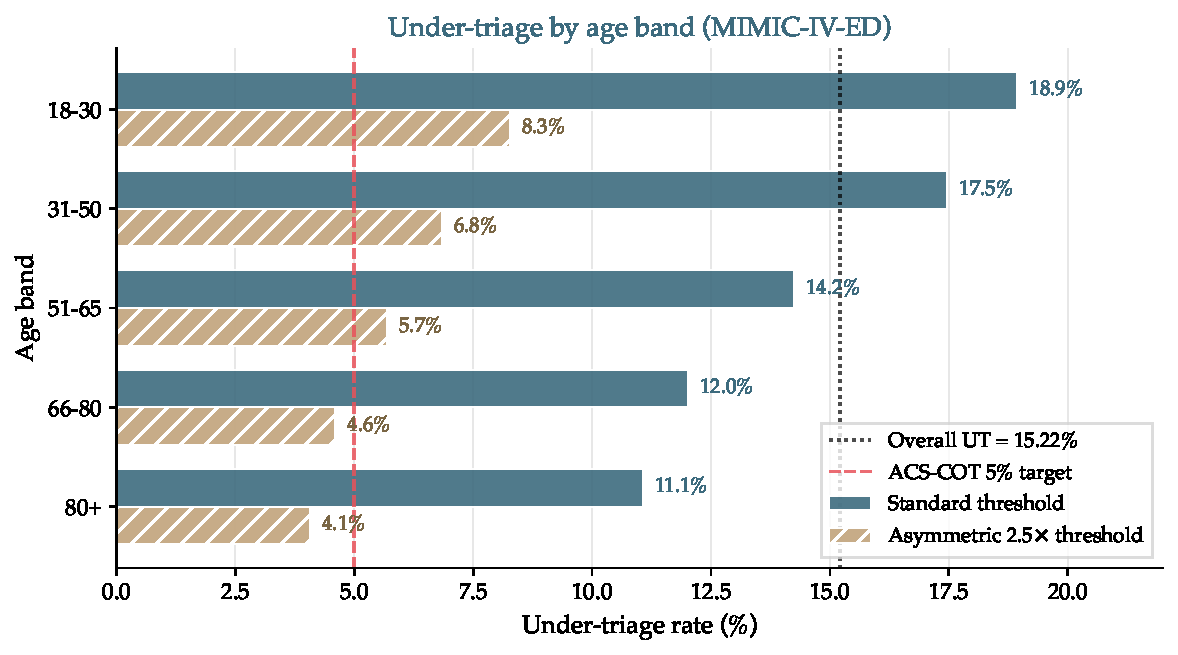
\includegraphics[width=\textwidth]{figures/bias_audit_disparities.pdf}
 \caption[Under-triage by age band]{Under-triage rate by age band on MIMIC-IV-ED,
shown at the default operating point (solid bars) and after applying the
asymmetric $2.5\times$ threshold from Chapter~\ref{ch:safety} (hatched bars).
The vertical black dotted line marks the overall under-triage rate ($15.22\%$);
the red dashed line marks the ACS-COT safety target ($5\%$). The monotonic
pattern (youngest bands under-triaged at the highest rate) is visible under
both thresholds. As discussed below, the safety intervention moves every
age band toward the target in absolute terms but increases the \emph{ratio}
between the best-served and worst-served bands. The figure shows age only;
sex and race subgroup rates are reported in Table~\ref{tab:single-axis} and
discussed in the surrounding text, with the caveat that the race mapping is
incomplete.}
 \label{fig:bias-audit}
\end{figure}

The implication is that the generic ``young'' category is under-triaged by the model, and this is visible regardless of how the other demographic axes are handled. The single-axis comparison in the next section makes the same claim in a cleaner form.

\section{Age Is the Dominant Axis}

To make the age-dominates-race finding precise, Table~\ref{tab:single-axis} reports the single-axis disparities.

\begin{table}[htbp]
 \centering
 \caption[Single-axis under-triage rates]{Under-triage rates broken down by one demographic axis at a time. Age shows the largest single-axis disparity: the youngest band has $1.71\times$ the under-triage rate of the oldest band. Race shows a smaller disparity of $1.30\times$ (subject to the mapping caveat above: HISPANIC and ASIAN categories in particular are substantially undercounted and their rates are preliminary). Sex is essentially null. Note that these rates are \emph{averaged over the other axes}: the per-axis disparities are smaller in magnitude than the disparities seen when the axes combine, which is the general reason intersectional audits are worth running.}
 \label{tab:single-axis}
 \small
 \begin{tabular}{lrrr}
 \toprule
 Axis value & N & UT rate & Severe UT \\
 \midrule
 \multicolumn{4}{l}{\textit{Age}} \\
 18--30 & 81{,}034 & 18.94\% & 0.90\% \\
 31--50 & 106{,}986 & 17.47\% & 0.74\% \\
 51--65 & 105{,}580 & 14.25\% & 0.46\% \\
 66--80 & 78{,}760 & 12.02\% & 0.32\% \\
 80+ & 45{,}665 & 11.07\% & 0.25\% \\
 \multicolumn{2}{r}{\textit{Max/min:}} & \multicolumn{2}{l}{\textbf{1.71$\times$}} \\
 \midrule
 \multicolumn{4}{l}{\textit{Sex}} \\
 F & 227{,}007 & 15.11\% & 0.55\% \\
 M & 191{,}093 & 15.34\% & 0.59\% \\
 \multicolumn{2}{r}{\textit{Max/min:}} & \multicolumn{2}{l}{1.02$\times$} \\
 \midrule
 \multicolumn{4}{l}{\textit{Race (aggregated; see caveat)}} \\
 HISPANIC & 3{,}070 & 18.73\% & 0.91\% \\
 ASIAN & 7{,}215 & 17.77\% & 0.87\% \\
 OTHER & 106{,}728 & 16.07\% & 0.62\% \\
 BLACK & 76{,}118 & 15.99\% & 0.57\% \\
 WHITE & 224{,}969 & 14.42\% & 0.53\% \\
 \multicolumn{2}{r}{\textit{Max/min:}} & \multicolumn{2}{l}{1.30$\times$} \\
 \bottomrule
 \end{tabular}
\end{table}

Age produces a $1.71\times$ disparity between the youngest and oldest bands. Race produces a $1.30\times$ disparity (with the caveat, again, that the HISPANIC and ASIAN categories are substantially undercounted and the race comparisons should be treated as preliminary). Sex produces essentially no disparity: $1.02\times$, well within sampling noise for a dataset of this size.

Much of the published clinical-ML fairness discussion has focused on race as the primary axis of concern, motivated by evidence that racial disparities exist in clinical outcomes and that models can amplify them; \citet{sax2023mistriage} report one such pattern in a large ED cohort, where under-triage rates were documented to differ between racial groups. On this cohort, my model shows a modest race disparity in the same direction, but the race effect is smaller than the age effect. For this population, and with the caveats noted above, age is the larger axis.

\begin{remarkbox}[Why This Matters for Fairness Audits]
I did not expect age to be the dominant axis. When I set up the bias audit, I was primarily watching race. The age effect became visible only when I looked at the full intersectional sweep and noticed that the subgroups with the highest under-triage rates consistently involved the 18--30 or 31--50 bands. This is a reminder that the axes that matter in a fairness audit are not always the axes one pre-registers for examination.

The broader discourse around algorithmic fairness in medicine tends to focus on race and, to a lesser extent, sex. These are important axes and should continue to be audited. But a thorough audit also benefits from examining age, language, insurance type, and other dimensions that may be less politically salient but no less consequential for individual patients. A 22-year-old man misclassified as ESI-3 when he should have been ESI-2 is not less harmed by that error than a 70-year-old woman in the same situation.
\end{remarkbox}

\section{Why Young Patients: Compensated Shock}

Why would my model under-triage young patients? The question admits of several possible answers, and distinguishing between them matters.

One possibility is that the labels themselves are biased. If triage nurses under-triage young patients (perhaps because youth is an implicit proxy for health in clinical intuition), then my model, trained to reproduce the labels, would inherit the bias. This is a common concern in medical ML.

Another possibility is that the features available to the model carry less predictive signal for young patients. If the relationship between vital signs and acuity is weaker in young patients than in old, then the model will be less confident about their true acuity, and its errors will concentrate there.

The clinical literature points strongly to the second explanation through a phenomenon called \emph{compensated shock}. In young healthy adults, the cardiovascular system maintains homeostasis aggressively in the face of physiological insult. A young person losing significant blood volume will maintain near-normal heart rate and blood pressure for substantially longer than an older person with the same injury, through vasoconstriction, increased cardiac output, and other compensatory mechanisms. The hemodynamic ``normal'' appearance conceals developing critical illness. This is one of the first things taught in Advanced Trauma Life Support training: young patients in shock often look deceptively stable.

\begin{notebox}[What Is Compensated Shock?]
In clinical terminology, shock is the state in which tissue perfusion is inadequate for metabolic demand. Classical presentations involve tachycardia (high heart rate), hypotension (low blood pressure), and altered mental status, the signs that prompt immediate escalation.

In the early stages, however, the body compensates. Baroreceptors detect the drop in pressure and trigger sympathetic activation: the heart beats harder and faster, peripheral arteries constrict to maintain central pressure, and oxygen delivery to critical organs is preserved. The result is a patient whose vital signs are within the normal range despite significant physiological derangement.

Young adults have considerable cardiovascular reserve and compensate more effectively than older patients. A 25-year-old can lose $30\%$ of their blood volume before their heart rate and blood pressure shift decisively outside normal range; an 80-year-old with the same loss would show abnormal vitals much earlier, because they have less reserve to draw on. The clinical implication is that ``normal vitals'' means different things at different ages: reassuring in an 80-year-old, potentially misleading in a 25-year-old.

Compensated shock is a well-established concept in trauma medicine, covered extensively in textbooks and in courses like Advanced Trauma Life Support. What is less well-studied is how machine learning triage systems handle it, because such systems are rare and their subgroup performance is rarely reported.
\end{notebox}

If compensated shock is the mechanism behind my age disparity, then I should be able to see it directly in the data. Specifically: among patients whose true ESI label is high-acuity (ESI-1 or ESI-2), what fraction present with vital signs in the normal range? If young patients are more likely to present with normal vitals despite being critically ill, I have a direct quantitative confirmation of the clinical intuition.

Figure~\ref{fig:compensated-shock} shows the analysis.

\begin{figure}[htbp]
 \centering
 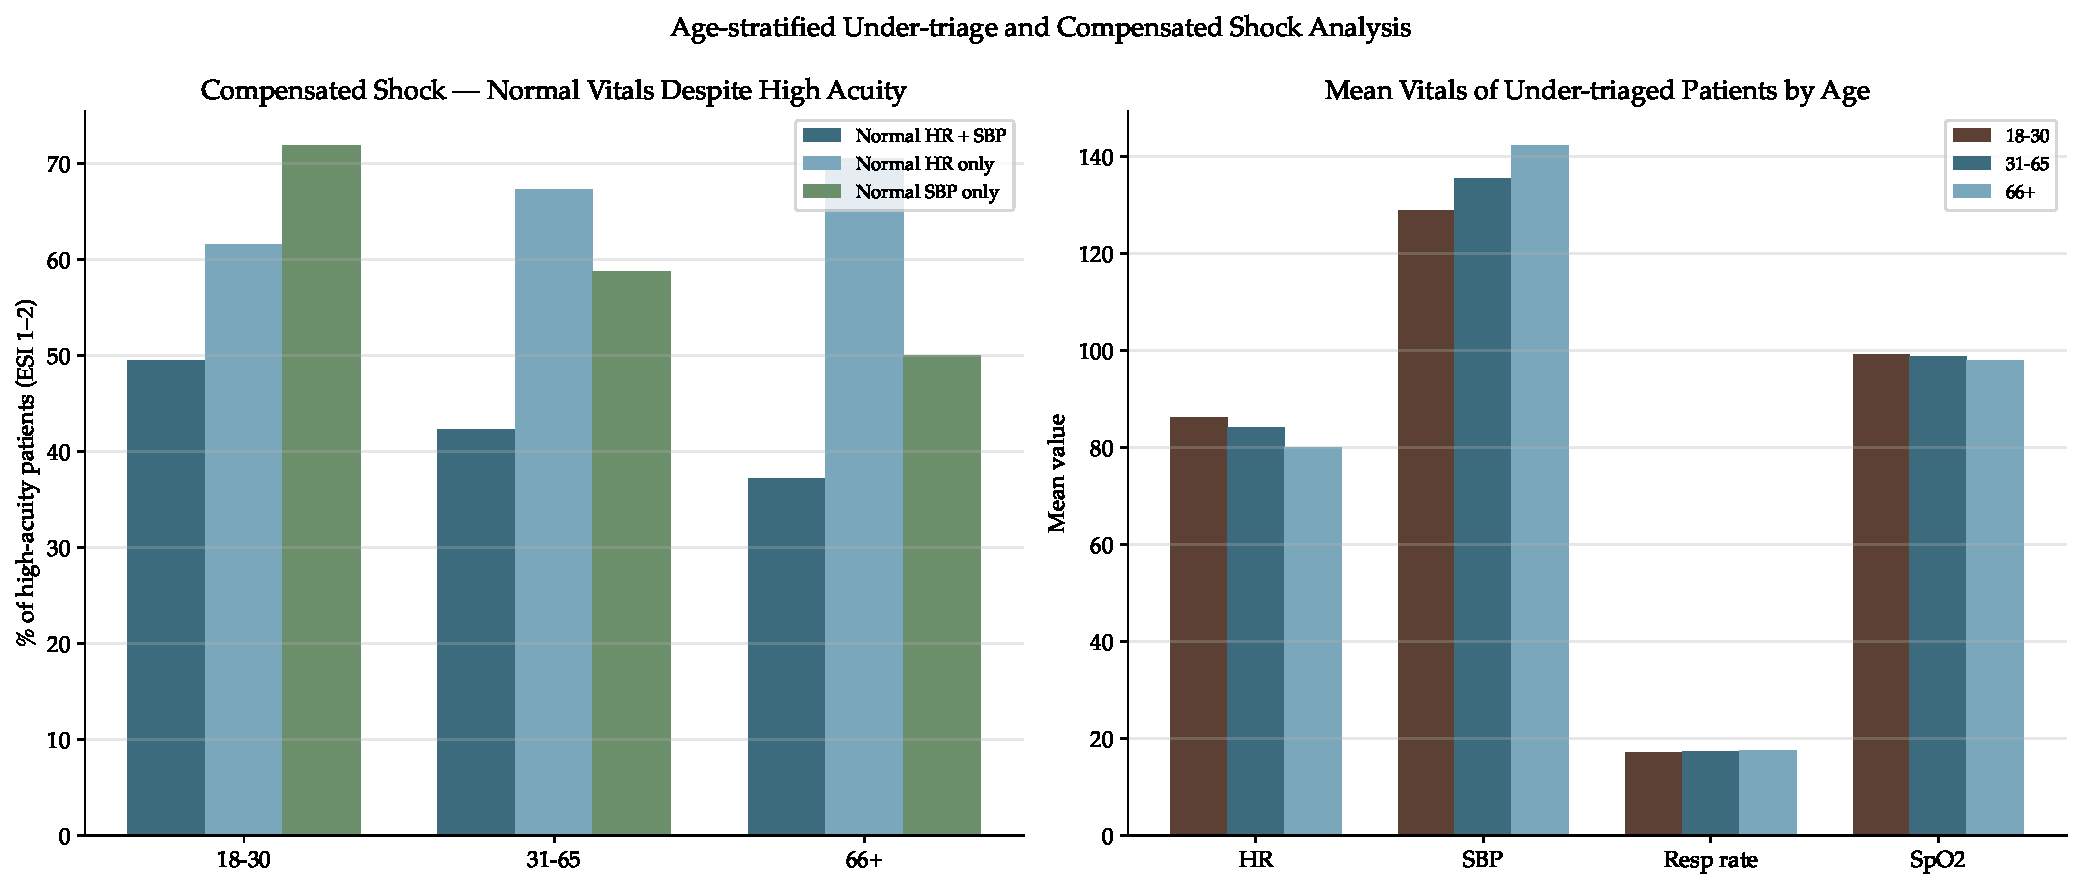
\includegraphics[width=0.95\textwidth]{figures/age_undertriage_vitals_comparison.pdf}
 \caption[Age-stratified vital sign patterns in high-acuity patients]{Left: the percentage of high-acuity patients (true ESI-1 or ESI-2) whose vital signs present in the ``normal'' range at triage, stratified by age band. The three conditions are: both heart rate and systolic BP within normal limits simultaneously; heart rate alone within normal limits; systolic BP alone within normal limits. The 18--30 group has the highest rate of normal presentation across all three measures, consistent with compensated shock masking critical illness. Right: mean values of four vital signs among under-triaged patients, stratified by age. Young under-triaged patients have mean values close to textbook normal, while older under-triaged patients show more deranged vital signs (lower HR, higher SBP, worse oxygenation).}
 \label{fig:compensated-shock}
\end{figure}

The numbers are striking. Among critically ill (ESI-1/2) patients aged 18--30, $49.48\%$ present with both heart rate and systolic blood pressure in the normal range. The same figure for patients aged 31--65 is $42.27\%$, and for patients aged 66+ it is $37.15\%$. Half of young critically ill patients at triage look, on the two main hemodynamic indicators, like healthy people.

The right panel of the figure shows mean vitals among patients the model under-triaged. Under-triaged 18--30 patients have mean heart rate $86.1$ bpm (squarely in normal range), mean systolic BP $128.8$ mmHg (normal), mean oxygen saturation $99.2\%$ (textbook), and mean temperature $98.1$°F (normal). These are the vital signs of apparently healthy people. The model classified them as lower acuity not because it made a careless mistake, but because their clinical presentations, on the features available, were consistent with lower acuity.

This is compensated shock, written into the MIMIC data in the pattern I would predict from the clinical literature. My model's age disparity is not a bias introduced by the modelling pipeline. It is an accurate reflection of a real clinical phenomenon: on the features available at triage, young critically ill patients look more like stable patients than old critically ill patients do.

I note the limitation: I am interpreting an empirical pattern in MIMIC-IV-ED through the lens of the compensated shock concept, but I have not independently validated the causal mechanism. A rigorous test would require linking patient outcomes, mortality, time-to-intervention, length of stay, to the vital sign patterns I observe, and demonstrating that the young patients I describe as ``compensated'' were indeed more critically ill than their vitals suggested. I did not do this analysis. The interpretation I offer is the most parsimonious explanation of the pattern I observe, grounded in well-established clinical knowledge, but further work is needed to confirm it.

\section{Can Feature Engineering Fix This?}

If compensated shock is the mechanism, the natural intervention is to engineer features that expose it. Raw vital signs are age-blind: a heart rate of $95$ is just a heart rate of $95$. A vital sign \emph{expressed relative to age-specific norms} might better flag the young patient whose nominally-normal heart rate is actually mildly elevated for their demographic.

I constructed a set of age-adjusted features:

\begin{itemize}
 \item \texttt{hr\_age\_zscore}, \texttt{sbp\_age\_zscore}, and so on: z-scores of each vital sign relative to the mean and standard deviation within the patient's age decile, computed from the training fold.
 \item \texttt{n\_age\_abnormal\_vitals}: a count of how many of the patient's vitals fall more than two standard deviations from their age-decile mean.
\end{itemize}

Adding these twelve features to the base feature set produced the augmented pipeline described in Chapter~\ref{ch:features}. Because it is easier to run a clean ablation with a single model than with the full blend, I report single-model results here. The comparison is summarised in Table~\ref{tab:augmented}.

\begin{table}[htbp]
 \centering
 \caption[Augmented feature ablation]{Performance of a single-model pipeline with and without age-adjusted features. The augmented features close the age disparity substantially: under-triage among 18--30 patients drops from $18.94\%$ (baseline, single-axis, full blend) to $14.57\%$ (augmented single-model), bringing it close to the rates for older bands. F1 is essentially unchanged. These results are for a single-model pipeline; a fair blend-to-blend comparison with the full feature set was not saved and would be the natural follow-up.}
 \label{tab:augmented}
 \small
 \begin{tabular}{lcc}
 \toprule
 & Baseline single-model & Augmented single-model \\
 & (65 features) & (77 features) \\
 \midrule
 Overall macro F1 & 0.556 & 0.557 \\
 Overall UT & (not saved) & 14.06\% \\
 \midrule
 UT, 18--30 & (not saved) & 14.57\% \\
 UT, 31--65 & (not saved) & 14.33\% \\
 UT, 66+ & (not saved) & 13.27\% \\
 \midrule
 Disparity ratio (18--30 / 66+) &, & 1.10$\times$ \\
 \bottomrule
 \end{tabular}
\end{table}

Two new features, \texttt{hr\_age\_zscore} at rank 11 and \texttt{n\_age\_abnormal\_vitals} at rank 15, appear in the top 20 by LightGBM gain importance, confirming that the model is using them. Figure~\ref{fig:feature-importance-aug} shows the feature importance comparison between baseline and augmented configurations.

\begin{figure}[htbp]
 \centering
 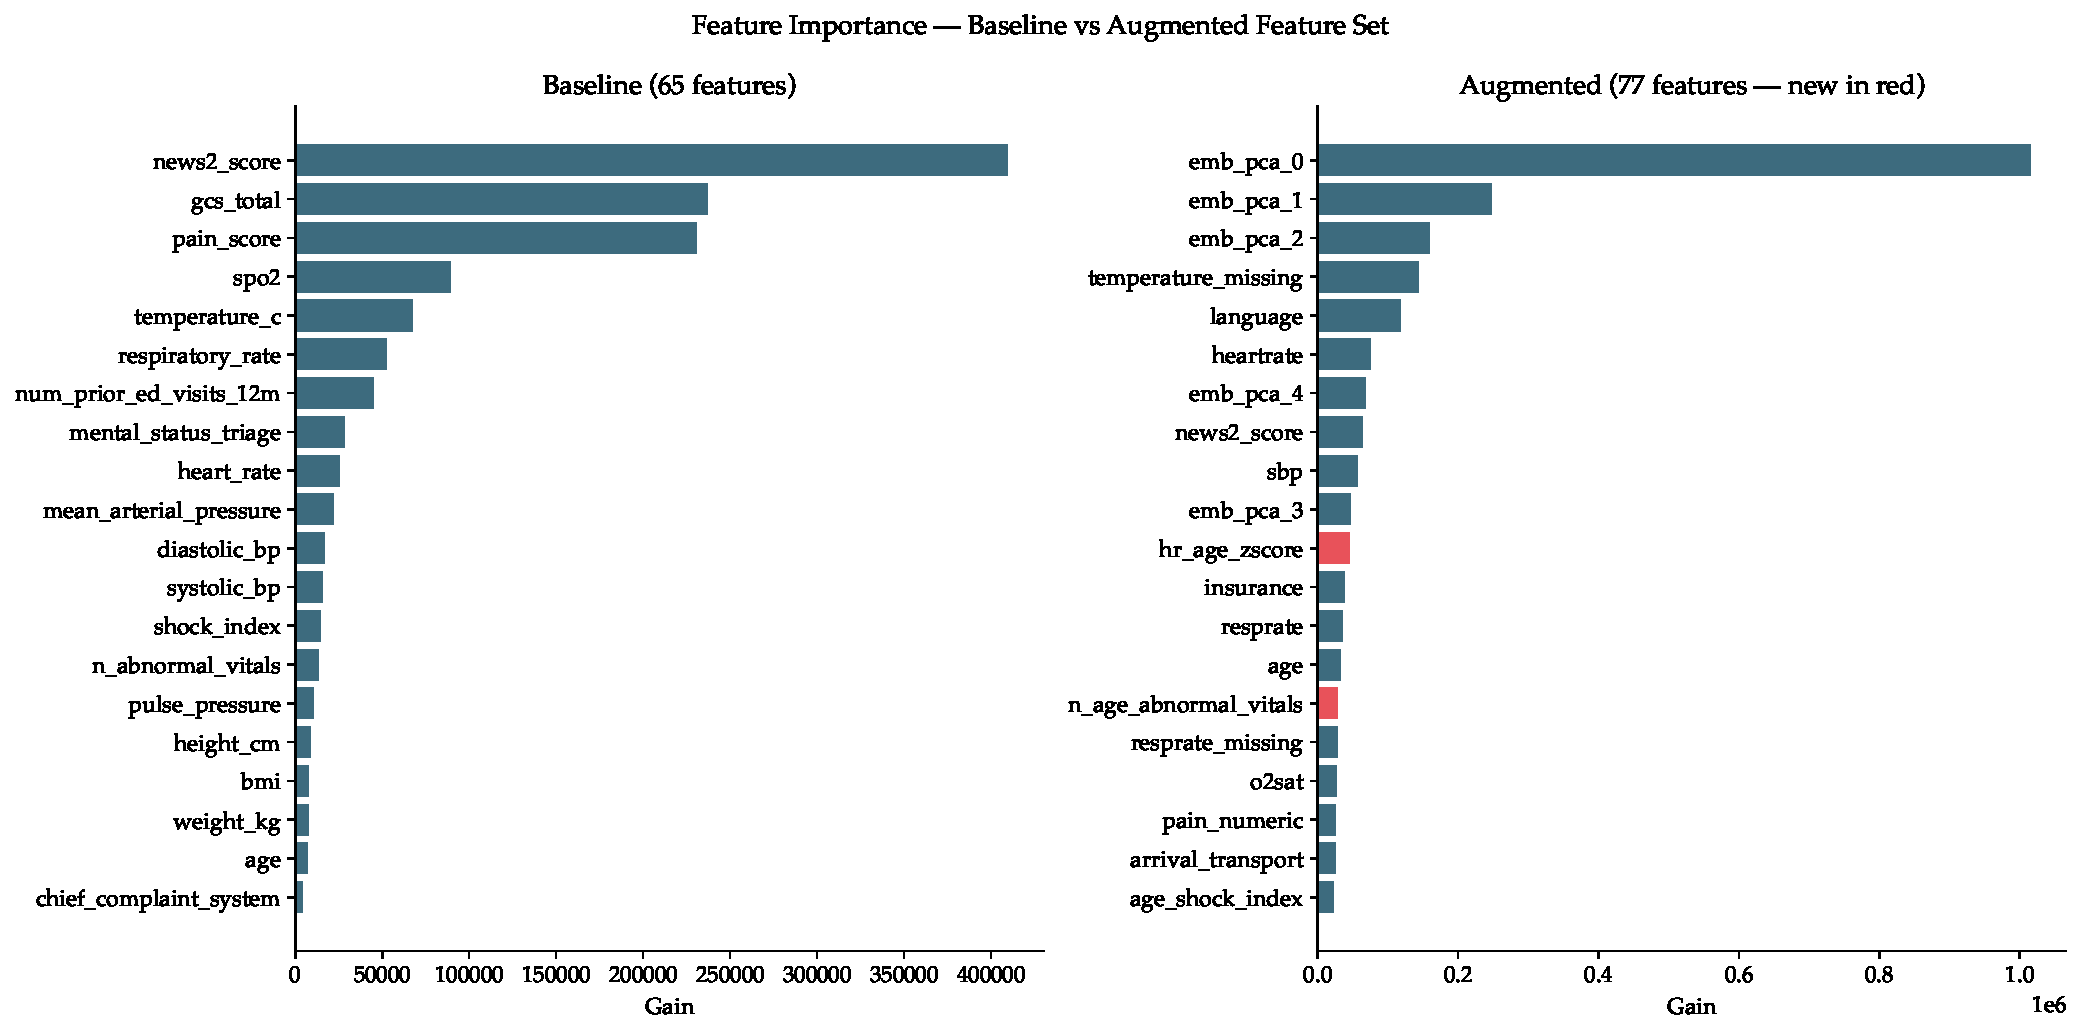
\includegraphics[width=\textwidth]{figures/feature_importance_augmented_vs_baseline.pdf}
 \caption[Feature importance: baseline vs augmented]{LightGBM gain importance for the top 20 features in the baseline 65-feature model (left) and the augmented 77-feature model (right). Two new age-adjusted features appear in the top 20 of the augmented model: \texttt{hr\_age\_zscore} at rank 11 and \texttt{n\_age\_abnormal\_vitals} at rank 15 (shown in red). The model uses these features substantially. The augmented model closes the age disparity to approximately $1.1\times$ from the baseline's $1.7\times$, while overall F1 is essentially unchanged.}
 \label{fig:feature-importance-aug}
\end{figure}

The augmented single-model closes the age disparity dramatically: the gap between 18--30 and 66+ under-triage rates falls from the baseline's $1.71\times$ ratio to roughly $1.10\times$. The overall F1 is essentially unchanged ($0.5569$ versus $0.5562$), within the noise of per-fold variation.

This is the most encouraging result of the chapter, and also the one that deserves the most caution in how it is interpreted. I emphasise two caveats.

First, this comparison is single-model, not blend-versus-blend. The blend pipeline's per-age-group UT rates were not saved for the baseline configuration, so I cannot report a clean apples-to-apples comparison at the blend level. The direction of the effect, age-adjusted features close the disparity, is robust, but the precise magnitude at the blend level would need to be re-run to verify.

Second, feature engineering is not a complete fix. A $1.10\times$ disparity is not zero. Young critically ill patients still present with deceptively normal vitals, and no amount of feature engineering can extract signal that is not there. What the age-adjusted features do is use the signal that \emph{is} there more efficiently: a heart rate of 95 for a 25-year-old is no longer treated the same as a heart rate of 95 for an 80-year-old. The remaining disparity is presumably the portion driven by genuinely ambiguous cases where the compensated shock is complete enough that no feature engineering can reveal it.

\section{The Safety Intervention Widens the Disparity}

I now return to a finding I flagged in passing during Chapter~\ref{ch:safety}. The asymmetric $2.5\times$ threshold intervention, which reduces the overall under-triage rate from $15.22\%$ to $6.10\%$, has a concerning effect when examined at the subgroup level.

At the standard threshold, the ratio between the worst-performing subgroup (the worst-off group in the bias audit) and the best-performing subgroup is $2.47\times$. After applying the asymmetric threshold, the ratio climbs to $3.15\times$. This is a $28\%$ widening of the relative disparity, even though every subgroup's absolute under-triage rate falls.

Figure~\ref{fig:bias-audit}, revisited, shows this pattern directly. Compare the solid (standard) to hatched (asymmetric) bars for each subgroup. The worst-served subgroups see their rates fall, but not by as large a proportion as the best-served subgroups. Concretely, across the full audit, the worst-served subgroup's rate falls from $22.3\%$ to $11.7\%$ (a $47\%$ relative reduction), while the best-served subgroup's rate falls from $9.1\%$ to $3.7\%$ (a $59\%$ relative reduction). The absolute gaps narrow; the relative gaps widen.

The intervention helps everyone in absolute terms, but helps the already-better-served more in relative terms. I do not name the specific demographic composition of the worst- and best-served subgroups here because, as noted above, the race mapping used in this audit is incomplete, and the relevant finding for the policy question below is the shape of the effect, not the identity of any particular group.

\begin{remarkbox}[Uniform Interventions Are Not Uniform in Effect]
This is a structural feature of cost-sensitive interventions applied to a well-calibrated classifier, not a quirk of my specific setup. When a threshold multiplier scales all classes proportionally, it moves all patients' predicted acuities upward, but the effect on each patient depends on where their predicted probabilities started. Patients whose probabilities were already borderline benefit most; patients deep in the wrong class do not benefit much at all.

Young critically ill patients with compensated shock are, by construction, not borderline, their feature values genuinely look like lower-acuity presentations. A threshold multiplier does not rescue them as effectively as it rescues old critically ill patients whose feature values already looked somewhat concerning. The multiplier is a uniform lever; the underlying classifier is not uniform in its confidence across subgroups; and therefore the effect of the lever is not uniform either.

The policy implication is that threshold-based safety interventions should be audited for subgroup disparity, not just overall performance. A hospital considering my $2.5\times$ multiplier should know that it widens the relative disparity between demographic subgroups, even as it improves absolute safety for every group.
\end{remarkbox}

I think this is one of the most important findings of the project, precisely because it is unexpected and would be easy to miss. A developer reporting only overall metrics, both overall UT and overall F1, would present the asymmetric threshold as an unambiguous improvement. The subgroup analysis reveals that the improvement is distributed unequally, and that the patients already least well-served by the model are the ones who benefit least from the safety intervention.

\section{Directions for a Complete Fairness Audit}

Several threads from this chapter deserve follow-up work that was not feasible within my timeline.

A proper race mapping should be constructed before any definitive claims about race disparities are made. My current mapping undercounts HISPANIC and ASIAN categories substantially; the race-level numbers in this chapter should be treated as preliminary rather than definitive.

The blend-level comparison of baseline versus age-adjusted features would complete the feature-engineering argument. The single-model comparison is suggestive but not conclusive; a full blend comparison with per-subgroup metrics saved would confirm or challenge the direction.

Outcome-based validation of the compensated shock interpretation would strengthen the causal claim. If young patients I identify as ``compensating'' indeed have more serious diagnoses or require more urgent interventions than their triage labels suggest, that would provide evidence beyond the vital-sign patterns I report here.

External validation across institutions would test whether the age-dominates-race pattern is specific to MIMIC-IV-ED or is a general feature of ED triage. Beth Israel Deaconess has a specific case mix, demographic distribution, and triage practice; the pattern might be different at a community hospital, a pediatric centre, or an institution in a different country.

Disparity audits at multiple operating points along the full Pareto frontier, rather than just two points, would give a more complete picture of how safety-accuracy trade-offs interact with subgroup fairness. I expect that some points on the curve might be more equitable than others, and identifying them could inform deployment decisions.

\section{What This Chapter Contributes}

The bias audit surfaces a pattern I did not expect: age is the dominant axis of variation in under-triage rate in this cohort, larger than race or sex. Patients aged 18--30 are under-triaged at $1.71\times$ the rate of the oldest band (80+). Subgroups combining young age with other demographic characteristics occupy the top of the distribution; race-specific claims within that set are not defensible on this data because of the incomplete race mapping discussed above.

The pattern is consistent with the clinical phenomenon of compensated shock. Among truly critically ill patients, $49.5\%$ of those aged 18--30 present with both heart rate and systolic blood pressure in the normal range; for patients aged 66+, this figure is $37.2\%$. Young patients in shock look more normal than old patients in shock, and my model sees this pattern as cleanly as any trained clinician would.

Age-adjusted features close the disparity substantially with essentially no cost in F1, confirming that the model can be made more equitable through feature engineering rather than through accuracy-vs-fairness trade-offs. This is the most encouraging finding of the chapter, but the comparison I present is single-model and would need to be replicated at the blend level.

The safety threshold intervention from Chapter~\ref{ch:safety} \emph{widens} the relative disparity between best- and worst-served subgroups, even as it reduces every subgroup's absolute under-triage rate. This is a policy-relevant finding: uniform thresholds have non-uniform effects across demographic groups, and safety interventions in clinical ML should be audited for this pattern.

The next chapter turns to explainability: how the model reaches its predictions, which features drive which classifications, and what this means in the context of the emerging EU AI Act requirements for high-risk medical systems. I have built a model that is, in aggregate, as reliable as human triage. I have characterised its trade-offs between accuracy and safety, and its disparities across demographic subgroups. What remains is to make its reasoning legible.
